\title{Chum Populations}

\documentclass[12pt,  one column]{article}
\usepackage{graphicx}
\usepackage{float}
\usepackage{enumitem}
\usepackage{natbib}

\begin{document}
% \bibliographystyle{}

\section*{Abstract}
None yet


\section*{Outline}
\begin{itemize}

\item Puget Sound chum salmon populations
\begin{itemize}
\item Population structure
\item chum salmon anadromous life history - 
\item ESA listing - summer chum ESU
\item Effective population size
\end{itemize}

\item Genotyping duplicates
\begin{itemize}
\item Legacy of the salmonid WGD
\item uncharacterized regions of the genome 
\item first approach in salmon using next-gen seq data.
\end{itemize}

\item Genome scan
\begin{itemize}
\item map-assisted
\item paired population design
\item draw on synteny / orthology to interpret results
\end{itemize}

\item Map
\begin{itemize}
\item consensus map
\item synteny
\item annotation
\end{itemize}

\end{itemize}

\pagebreak



\section*{Introduction}
\begin{itemize}

\item Puget Sound chum salmon populations
\begin{itemize}
\item Population structure
Wild distribution

Two Evolutionary significant units (ESU) - Hood canal summer vs the rest. 'Genetically and ecologically distinct' threatened under the ESA. Notice which populations where supplemented by hatchery programs?
Chum salmon stray at similar rates to other pacific salmon \cite{Small2014} (also could cite johnson et al 1997).

\item chum salmon anadromous life history - 
eggs deposited nov-dec
embryos devlop and hatch after ~4 months coupled with a migration to sea. 'survival and growth in juvenile chum salmon depend less on freshwater conditions than on favorable estuarine and marine conditions.'
return to spawn at 3-5 years of age, spawn within 100km of the ocean

\item life history variation
\item ESA listing - summer chum ESU
\item Effective population size
\end{itemize}

\item Genotyping duplicates
\begin{itemize}
\item Legacy of the salmonid WGD
\item uncharacterized regions of the genome - retained through unknown mechanisms. Possible benefits are unknown but could include reduced inbreeding depression in small isolated populations typical of salmonids.
\item This is the first time that high-throughput sequencing data has been applied to score duplicated loci within salmonids.
\end{itemize}

\item Genome scan
\begin{itemize}
\item map-assisted
\item paired population design
\item draw on synteny / orthology to interpret results
\end{itemize}

\item Map
\begin{itemize}
\item A consensus linkage map was constructed from three gynogenetic haploid families (sizes 175, 4x, 3x). This linkage map is novel but builds on the map presented in \citet{Waples2015} with the addition of two additional families.  Within each linkage group, we estimate the location of the centromere (cite morten?).  

Paralogous loci were identified by through their segregation patterns as in \citet{Waples2015}.  At each locus, the observed allelic segregation pattern were fit to multiple models specified by 

\item The othologous loci and 
\item annotation
\end{itemize}

\end{itemize}


\section*{Methods}

\subsection*{Population Genetics}
\subsubsection*{Sequence analysis and genotyping}
\begin{itemize}[nosep]
\item Varaint SNPs were identified and genotyped with a reference-based approach with the Stacks software pipeline \cite{Catchen2013}.  Reference constructed from \citet{Waples2015}
\item alignment with BWA-mem, remove low-quality alignments
\item identify variants and assign genotypes with pstacks
\item filter genotypes and individuals to produce final data set. 
\item Does allelic bias filtration have a place here?
\end{itemize}

\subsubsection*{Individual-based analyses} 
\begin{itemize}[nosep]
	\item Genotyping duplicate loci using the dominance coding suggested by \cite{Patterson2006}. 
Individual-based analyses
	\item PCAs - How do these two methods compare? - maybe measure info loss?
    Use a Procrustes analysis to find an optimal transformation.  This allows the superimposition of one result onto another set of axes, through rotation and stretching.  produced a procrustes similarity \cite{Peres2001}.  Other option is a CCA (canonical correlation analysis)  
    \item Formal tests for population structure - tracey-widom stats.  Breakdown of population structure and lower PC axes

\end{itemize}

\subsubsection*{Population-based analyses} 

\begin{itemize}[nosep]
	\item MAF, Heterozygosity
    \item phylogenetic tree
    \item Genome scan - gloabal or paired populations - 	
    \item Fst across the genome.  Use LOESS (local regression) to reveal regions of elevated differentation.  Benefits of this approach vs a bootstrapping methods (eg. Hohenlohe 2010)
    \item Effective population size - 

    	Effective population size was estimated for each population using the LD method implemented in the LDNe software package \cite{Waples2010}.  The LD methods estimates average correlation of alleles at pairs of loci (r2). The mean pairwise r2 value across unlinked loci provides an estimate of contemporary effective population size. The linkage map was used to ensure that only pairs of loci not co-located on a chromosome were used to calculate mean r2.
        
Run this with and without the linkage map correction \cite{Larson2014}?

\end{itemize}

\subsection*{Linkage map}

Sequence analysis and genotyping

%Identification of paralogs follows \cite{Waples2015}

Map construction follows McKinney (2015), Waples (2015)

Synteny - relation to genetic resources
\begin{itemize}[nosep]
	\item Chinook salmon
    \item Atlantic salmon
\end{itemize}





\pagebreak
\section*{Results}

Genotyping rate
\subsection*{Population Genetics}
population structure

Summarize population relationships, consistent with \citet{Small2014}?

Four individual-based PCA figures

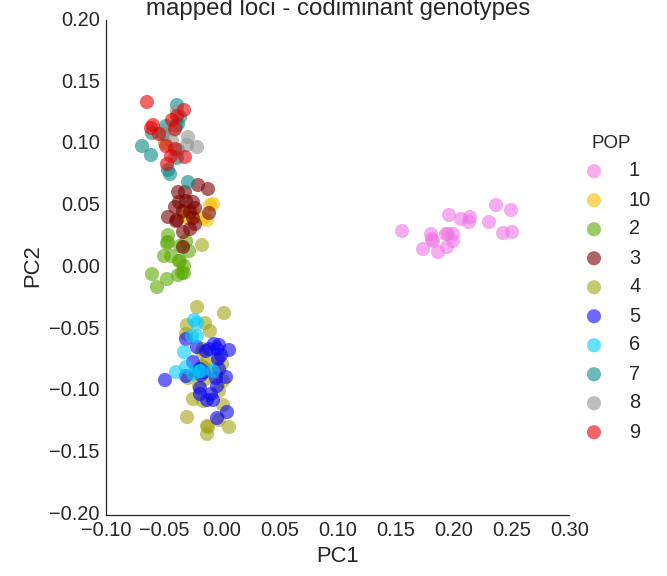
\includegraphics[scale=.3]{figures/PCA_codom.png}
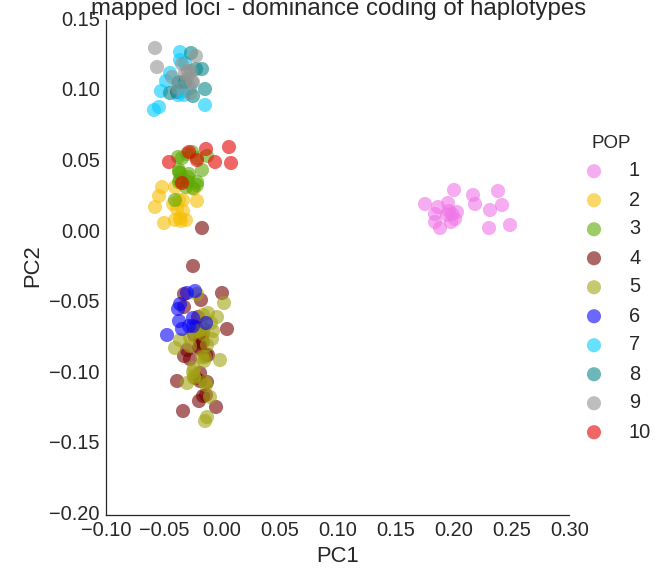
\includegraphics[scale=.3]{figures/PCA_dom.png}

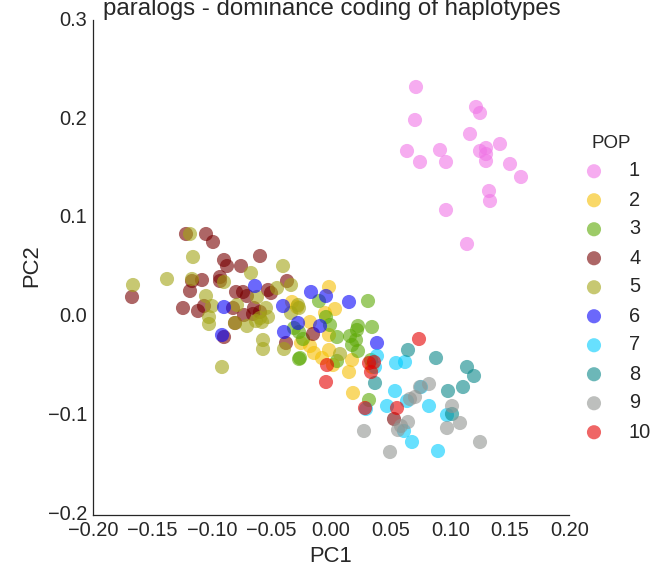
\includegraphics[scale=.3]{figures/PCA_dom_paralogs.png}
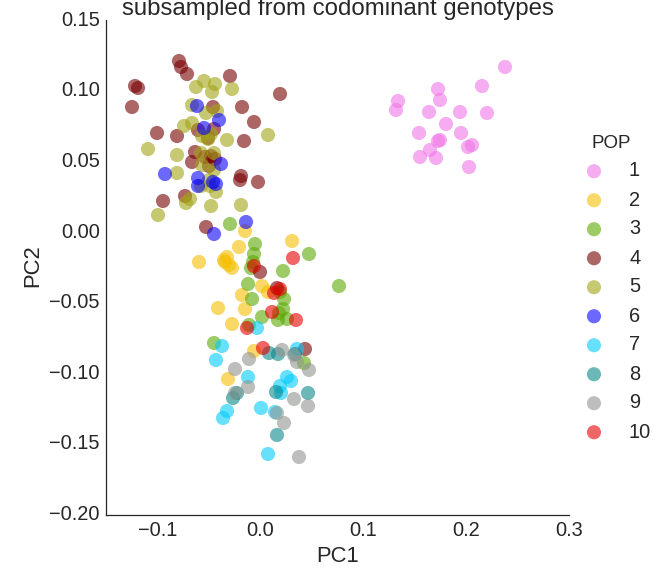
\includegraphics[scale=.3]{figures/PCA_codom_subsample.png}
Paralogs have similar neutral patterns of population structure (Procrustes similarity xxx)

Is the a possible quantitative measure of information loss due to dominance coding?  These doesn't quite make sense, as the the dominant haplotypes contain *more* information.

discuss population vs individual based results

can we demonstrate contained within paralogs by bootstrapping 
Genome scans - LG regions highlighted.

\subsection*{Effective population size}


Perhaps run the Ne with and without the linkage map correction?

\subsection*{Ascertainment Bias}
The linkage map was constructed from three female parents from Hoodsport hatchery, WA.

Demonstrate ascertainment effect when using only loci on linkage map - effect on allele frequencies.

\begin{figure}[H]
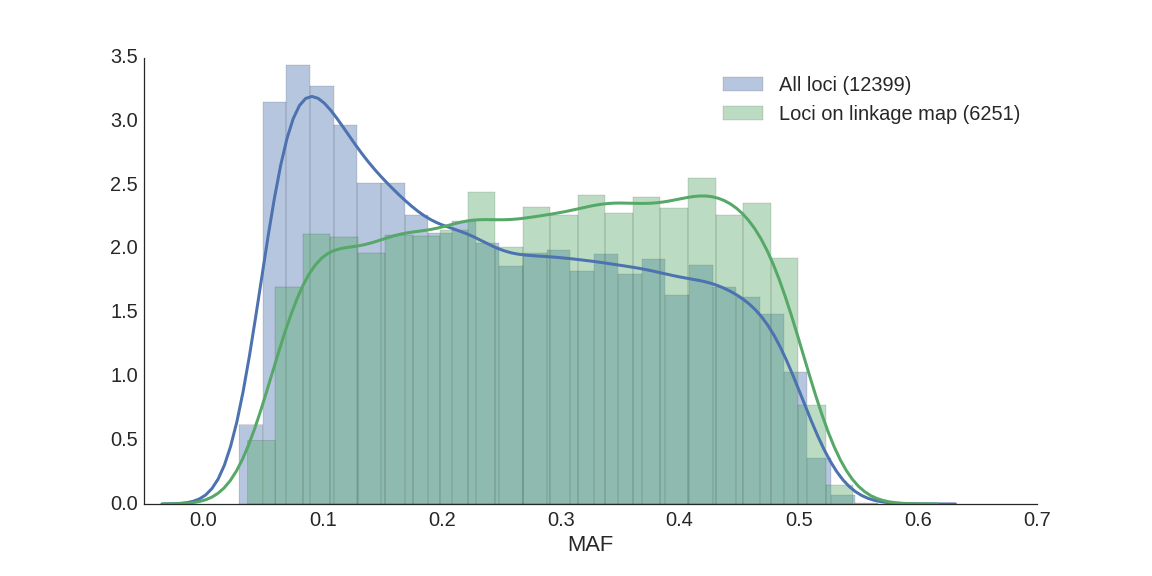
\includegraphics[scale=.3]{figures/supplemental/ascertainment.png}
\caption{Minor allele frequency (MAF) density histograms for all loci (blue) and the subset of loci placed on the linkage map (green). The rightward shift in the MAF distribution shows the effect of ascertainment bias.} \textbf{TODO: align histogram bins, check the .5 boundary}
\end{figure}

\subsection*{Linkage map}
Here we present a consensus map placing XXX loci onto 37 linkage groups.  These 37 linkage groups likely have a 1:1 correspondence with the 37 chromosomes in chum salmon. \textbf{Do we want a map figure, or just a table?}

A total of xxx paralogs were identified and placed onto the linkage map.  The location of these paralogs were were concentrated on the distal ends of three chromosomes, consistent with Identification of paralogs, congruence of identified homeologs across families (supplemental table)

placement of centromeres

paralogs

Notice the distribution of paralogs matches the  pattern found in other salmonids.
syntenic/orthologous relationships - per LG
Table (supplemental?)

\section*{Discussion}
To do

Compared to \citet{Small2014} the effective sizes (N$_{e}$) are larger, this could be due to the downward bias removed by utilizing the linkage map. 

Does this turn into two papers?

 - linkage map and individual-based analyses - including duplicated loci

 - inference of adaptation -associated  life history variation  - Fst across the genome.

\pagebreak
\section*{Supplemental}



\begin{figure}[H]
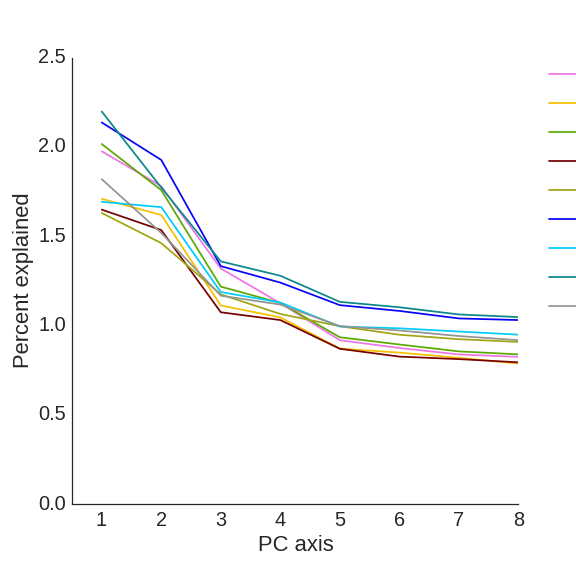
\includegraphics[scale=.4]{figures/supplemental/PCA_eigenvalues.png}
\caption{Percent variance explained (eigenvalue) for the first eight PC axes of each locus set.  Notice the similarity between the two bi-allelic sets and the two haplotypic sets.}
\end{figure}

\begin{figure}[H]
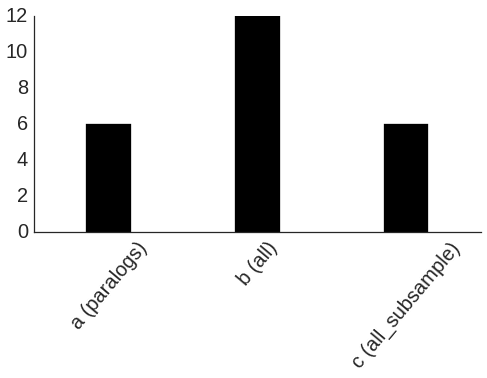
\includegraphics[scale=.4]{figures/supplemental/TW_stats.png}
\caption{Number of significant PC axes as determined by the Tracey-Widom test.}
\end{figure}

\begin{figure}[H]
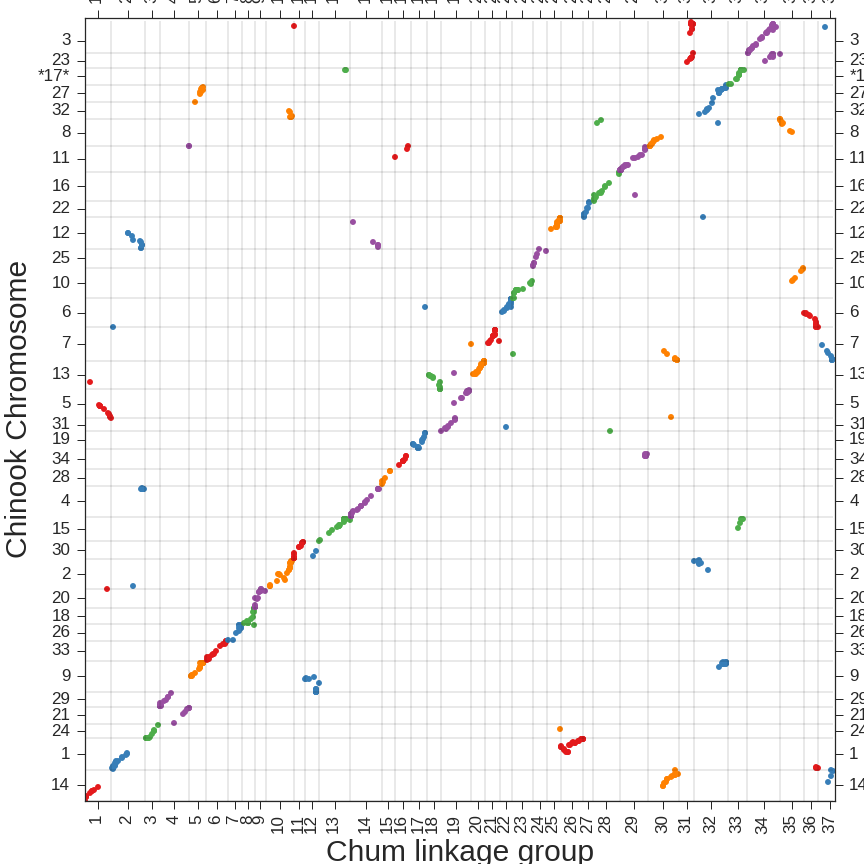
\includegraphics[scale=.25]{figures/supplemental/synteny_chinook.png}
\caption{Oxford grid - Chum and Chinook linkage groups.  Loci are positioned according to the order within each genome.}
\end{figure}

%\begin{figure}
%\begin{center}
%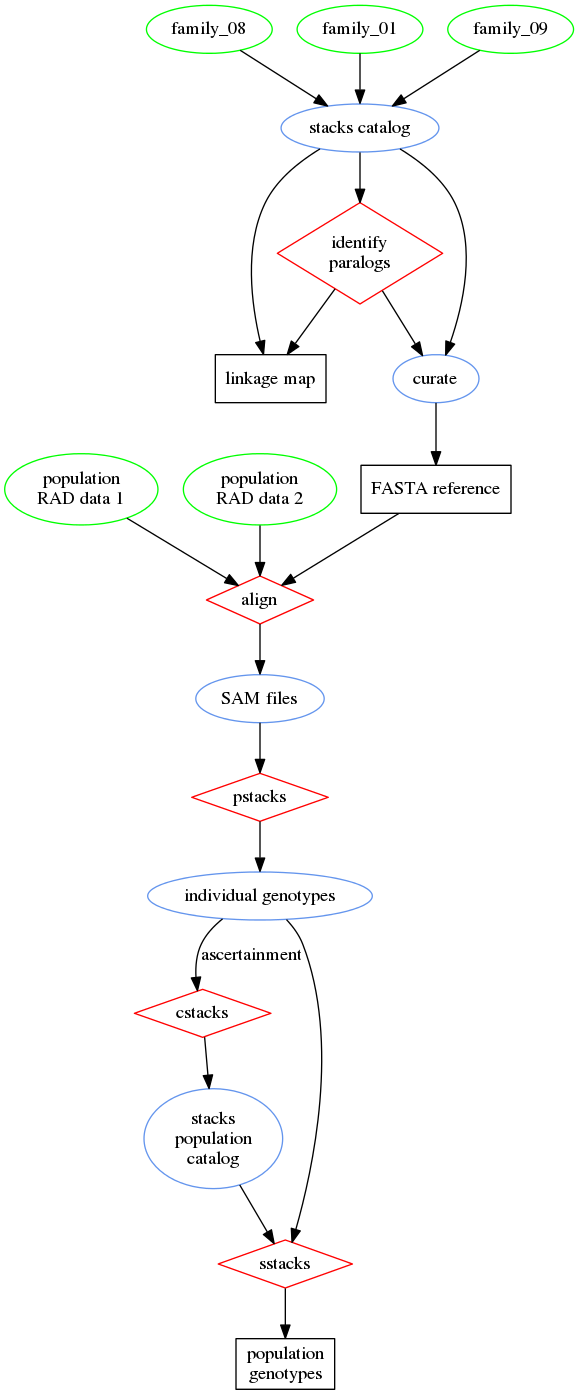
\includegraphics[scale=.3]{figures/supplemental/analysis_flowchart.png}
%\end{center}
%\end{figure}

\section*{Reference}

\bibliographystyle{apalike}
\bibliography{./bibtex/7_13_15}

\section*{Acknowledgements}
Rachel Hovel - advice woth multivariate stats.

\end{document}